\documentclass[t]{beamer}
\usepackage[brazil]{babel}
\usepackage[utf8]{inputenc}
\usepackage{graphicx,hyperref,url,pgfplots}
\usetheme{Warsaw}
% \usecolortheme{crane}
%\usefonttheme[onlymath]{serif}
\usefonttheme{professionalfonts}
% previsualização animacao
\setbeamercovered{invisible}
% texto justificado
\usepackage{ragged2e}
\justifying

\pgfplotsset{compat=1.10} 
\usepackage{amsmath} 
\usepackage{array,booktabs}

% tipos de slides
\newcommand{\pausar}{\pause}

% paginas numero
\addtobeamertemplate{navigation symbols}{}{%
    \usebeamerfont{footline}%
    \usebeamercolor[fg]{footline}%
    \hspace{1em}%
    \insertframenumber/\inserttotalframenumber
}

\usepackage{listings}
	\definecolor{codegreen}{rgb}{0,0.6,0}
	\definecolor{codegray}{rgb}{0.5,0.5,0.5}
	\definecolor{codepurple}{rgb}{0.58,0,0.82}
	\definecolor{backcolour}{rgb}{0.92,0.92,0.92}
	\lstset{language=Python, 
	backgroundcolor=\color{backcolour},   
	commentstyle=\color{codegreen},
	keywordstyle=\color{magenta},
	numberstyle=\tiny\color{codegray},
	stringstyle=\color{codepurple},
	basicstyle=\fontsize{8}{11}\ttfamily,
	frame=lines,
%	numbers=left,
	tabsize=2,
	morekeywords={models, lambda, forms}}

\logo{
\includegraphics[scale=0.09]{images/logo.jpg}}
\newcommand{\nologo}{\setbeamertemplate{logo}{}} % command to set the logo to nothing

\title[\textit{Introdução à robótica móvel}]{
  Cinemática Direta}

% Optional: a subtitle to be dispalyed on the title slide
\subtitle{Descrição espacial e Transformações}

% The author(s) of the presentation:
%  - again first a short version to be displayed at the bottom;
%  - next the full list of authors, which may include contact information;
% \author[Professor: Jeferson José de Lima]{
%   \textbf{Professor}: Jeferson José de Lima \\\medskip
%   {\small \url{jefersonlima@utfpr.edu.br}}}

  \author[Professor: Jeferson José de Lima]{
	\textbf{Professor}: Jeferson José de Lima}

% The institute:
%  - to start the name of the university as displayed on the top of each slide
%    this can be adjusted such that you can also create a Dutch version
%  - next the institute information as displayed on the title slide
\institute[UTFPR-PB]{
  Departamento de Informática (DAINF)}

% Add a date and possibly the name of the event to the slides
%  - again first a short version to be shown at the bottom of each slide
%  - second the full date and event name for the title slide
\date[2017.1]{\textbf{Disciplina}: Robótica Móvel}

\begin{document}

\begin{frame}
  \titlepage
\end{frame}

\begin{frame}
	\frametitle{Sumário}
	{\small {\small \tableofcontents}}
\end{frame}

% Section titles are shown in at the top of the slides with the current section 
% highlighted. Note that the number of sections determines the size of the top 
% bar, and hence the university name and logo. If you do not add any sections 
% they will not be visible.

\section{Informações Úteis}
\begin{frame} 
	\frametitle{Informações Úteis}
	\begin{block}{Material disponível em:}
		\href{Robótica Móvel - Wiki}{https://gitlab.com/cursoseaulas/robotica-movel/-/wikis/home}
	\end{block}
	\pausar
	\begin{alertblock}{Datas Importantes}
		\begin{itemize}
		\item Entrega
		\item Envio
		\end{itemize}
	\end{alertblock}
	\pausar
	\begin{exampleblock}{Requisitos da Disciplina}
		\begin{itemize}
		\item Teoria de Controle
		\item Linguagem de Programação - \textbf{Python} ou \textbf{C++}
		\item Eletrônica
		\end{itemize}
	\end{exampleblock}
\end{frame}

%-----------------------------------------------------------------
\section{Sistema de Coordenada}
\subsection{Sistema Coordenadas Universais}
\begin{frame}[c]
	\begin{center}
		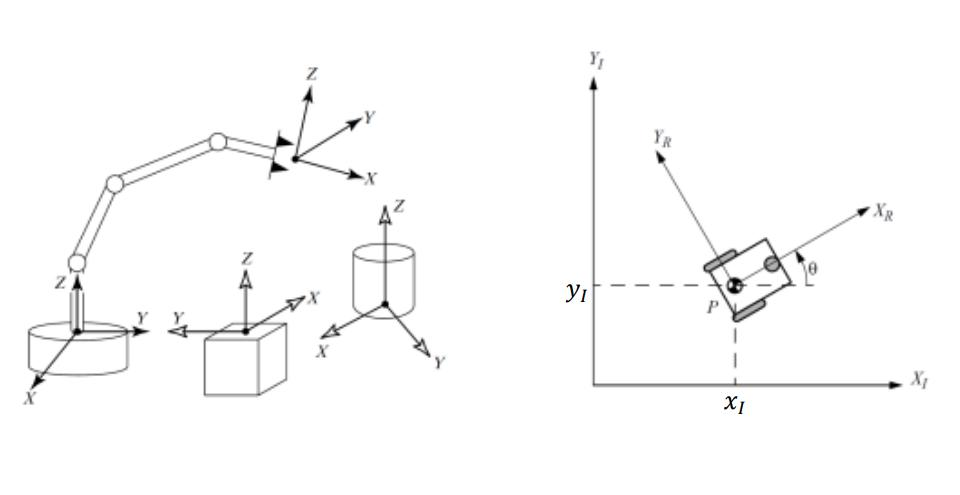
\includegraphics[width=0.8\textwidth]{images/mecanismos.jpg}
	\end{center}
\end{frame}
%%-----------------------------------------------------------------

\begin{frame}[c]
	\begin{itemize}
		\item coordenada como um vetor de posição $\mathbb{R}^{3 \times 1}$, composto pelas coordenadas $X,Y$ e $Z$.
		\item um ponto ${}^A\mathbf{P}$ representa a distância ao longo dos eixos do plano $\{A\}$. Os elementos individuais de ${}^A\mathbf{P}$ podem ser visto pela equação \eqref{eq:cine1}.
	\end{itemize}

	\begin{columns}[c]
			\begin{column}{0.6\textwidth}
			\begin{figure}
				\centering
				\begin{tikzpicture}[scale=0.6]]
				\node(p0) at (0,0){};
				\draw [->] (p0.center) --++(0,3) node[right] {$ Y_A$};
				\draw [->, rotate =120] (p0.center) --++(0,3) node[below] {$ Z_A$};
				\draw [->, rotate =240] (p0.center) --++(0,3) node[below] {$ X_A$};
				\draw [->] (p0.center) --++(2.5,0.5) node(B)[above,rotate=30] {${}^A\mathbf{P}$};
				\node at (-1.5,2.5) {$\{A\}$};
				\end{tikzpicture}
				\caption{Vetor em relação ao plano $\{A\}$}
				\label{fig:cine1f}
				\end{figure}
		\end{column}
		\begin{column}{0.4\textwidth}
			\begin{equation}\label{eq:cine1}
				{}^A\mathbf{P} = \begin{bmatrix}
				p_x\\ p_y \\ p_z
				\end{bmatrix}.
				\end{equation}			
		\end{column}
	\end{columns}

\end{frame}
%%-----------------------------------------------------------------
\begin{frame}[t]
	\begin{itemize}
		\item O vetor definido por ${}^A\mathbf{P}$ pode ser rotacionado pela matriz de rotação $\mathbf{R}$, conforme a equação \eqref{eq:cine2}.

		\begin{equation}\label{eq:cine2}
			{}_A^B
			\mathbf{R} = 
			\begin{bmatrix}
			r_{11} & r_{11} & r_{11}\\
			r_{21} & r_{21} & r_{21}\\
			r_{31} & r_{31} & r_{31}\\
			\end{bmatrix}
			\end{equation}
	
	\end{itemize}

	\begin{exampleblock}{Considera os exemplos}
		\begin{equation*}
			\mathbf{R}(\theta) = 
			\begin{bmatrix}
				\cos \theta &-\sin \theta \\\sin \theta &\cos \theta
			\end{bmatrix}
			\end{equation*}
		e igual:
		\begin{equation*}
			\mathbf{R}_z(\theta) = 
			\begin{bmatrix}
			\cos(\theta) & \sin(\theta) & 0\\
			\sin(\theta) & \cos(\theta) & 0\\
			0 & 0 & 1\\ 
			\end{bmatrix}
			\end{equation*}
	\end{exampleblock}

\end{frame}
%%-----------------------------------------------------------------

\begin{frame}[t]
	\begin{itemize}
		\item O vetor definido por ${}^A\mathbf{P}$ pode ser rotacionado pela matriz de rotação $\mathbf{R}$, conforme a equação \eqref{eq:cine2}.

		\begin{equation}\label{eq:cine2}
			{}_A^B
			\mathbf{R} = 
			\begin{bmatrix}
			r_{11} & r_{11} & r_{11}\\
			r_{21} & r_{21} & r_{21}\\
			r_{31} & r_{31} & r_{31}\\
			\end{bmatrix}
			\end{equation}
	
	\end{itemize}


\end{frame}
%%-----------------------------------------------------------------

\begin{frame}[c]
	\textbf{PIC ou Arduino?}
	\begin{center}
		
\includegraphics[width=1.3\textwidth]{images/logo.jpg}
	\end{center}
\end{frame}
%-----------------------------------------------------------------

\begin{frame}[fragile]
	\frametitle{Exemplo codigo}
		Comando \textit{while}: Enquanto(Sentença):
		\begin{lstlisting}
			int i=0;
			while (i <= 10){
				...
				i=i+1;
			}
			i=0;
		\end{lstlisting}
			Comando \textit{for}: repita até(Sentença):
		\begin{lstlisting}language=C]
			int i=0;
			for (i=0;i<=10;i++){
				...
			}
		\end{lstlisting}
\end{frame}

%-----------------------------------------------------------------
\begin{frame}[fragile]
	\frametitle{Exemplo codigo}
	Comando \textit{while}: Enquanto(Sentença):

	\begin{lstlisting}[language=Python]
		import numpy as np
		
		def incmatrix(genl1,genl2):
			m = len(genl1)
			n = len(genl2)
			M = None #to become the incidence matrix
			VT = np.zeros((n*m,1), int)  #dummy variable
			#compute the bitwise xor matrix
			M1 = bitxormatrix(genl1)
			M2 = np.triu(bitxormatrix(genl2),1) 
			... 
	\end{lstlisting}
\end{frame}


\begin{frame}[fragile]

	\begin{lstlisting}[language=Python]
			... 
			for i in range(m-1):
					for j in range(i+1, m):
						[r,c] = np.where(M2 == M1[i,j])
						for k in range(len(r)):
							VT[(i)*n + r[k]] = 1;
							VT[(i)*n + c[k]] = 1;
							VT[(j)*n + r[k]] = 1;
							VT[(j)*n + c[k]] = 1;
							if M is None:
								M = np.copy(VT)
							else:
								M = np.concatenate((M, VT), 1)
							VT = np.zeros((n*m,1), int)
		return M
	\end{lstlisting}
\end{frame}

%-----------------------------------------------------------------
\begin{frame}[allowframebreaks]

\textbf{Referências}

\begin{itemize}
\begin{small}
\item http://www.embarcados.com.br/arduino-entradasaidas-digitais/
\end{small}
\end{itemize}
\end{frame}
%-----------------------------------------------------------------
\end{document}
